\subsection{Empfangen der Messwerte}
 
\subsubsection{Python-Client für BLE-Verbindung}
\label{BLE_Python_Client}
Der Client wurde in Python geschrieben, da die Programmiersprache zum einen leicht zu verwenden ist und zum anderen wird von Adafruit die Bibliothek ,,Adafruit\_Python\_BluefruitLE'' zum Verbindungsaufbau mit BLE-Modulen bereitgestellt. Durch die beigefügten Beispiele hätte der Verbindungsaufbau mit dem Laptop einfach zu realisieren und somit eine Echtzeitdarstellung der ankommenden Daten möglich sein sollen. Vorher nicht bekannt war jedoch der Entwicklungsstand sowie der geringe Funktionsumfang dieser Bibliothek. Da in der kurzen Zeit keine Möglichkeit gefunden werden konnte, basierend auf diesen Klassen eine BLE-Verbindung aufzubauen, wurde mit der Entwicklung einer Alternative begonnen.

\subsubsection{Alternativer Client zum Empfang der Daten per BLE: Android-App}
\label{AndroidAppFürDatenmessen}
Da es bereits die Android-App ,,Adafruit Bluefruit LE Connect'' gibt, mit der Daten per Bluetooth empfangen und gesendet werden können, konnte davon ausgegangen werden, dass in der Konstellation Smartphone-Bluefruit-Modul BLE-Verbindungen funktionieren und unterstützt werden. Daraus ergibt sich sogar der Vorteil, dass ein Smartphone als Empfänger wesentlich mobiler ist, um an der Anlage am Sender mitlaufen zu können. 

Von Adafruit gibt es über Github\footnote{Github-Link: \url{https://github.com/adafruit/Adafruit_Android_BLE_UART}, 25.06.2016} die Klasse ,,Adafruit Android BLE UART'', mit der eine BLE-Verbindung zwischen einem Bluefruit-Modul und einem Android-Smartphone hergestellt werden kann. Dabei handelt es sich um eine abgespeckte Variante der oben erwähnten App. Basierend auf dem Quellcode für BLE-UART-Verbindungen wurde eine eigene App entwickelt. Als Entwicklungsumgebung kam Android Studio zum Einsatz. Neben dem Verbindungsaufbau muss die App Befehle an den Mikrocontroller senden können. Sobald Sensordaten vom Mikrocontroller ankommen, sollen diese Werte in lokalen Dateien gespeichert werden.

Zuerst musste eine Verbindung mit dem Bluefruit-Modul hergestellt werden. Bei eingeschaltetem Bluetooth am Smartphone sucht die App automatisch nach BLE-fähigen Geräten in der Nähe. 

Die App verfügt über vier Buttons, um das Verhalten des Mikrocontrollers sowie das Speichern der Daten kontrollieren zu können:
\begin{description}
	\item[Start:] Sendet einen Start-Befehl an den Mikrocontroller, damit dieser mit dem Senden von gemessenen Sensordaten beginnt.
	\item[Stop:] Sendet einen Stop-Befehl an den Mikrocontroller, damit dieser mit dem Senden von gemessenen Sensordaten stoppt. Die gemessenen Daten bleiben dabei in einem StringBuffer vorhanden.
	\item[Save:] Speichert die gemessenen Daten in einer neuen Datei ab. Dabei werden genutzte Zähler nicht zurückgesetzt. Der Button kann benutzt werden, um bei einem Messlauf markante Punkte auf der Sortieranlage zu markieren, indem eine neue Datei erstellt wird. Zusätzlich wird mit dem Zwischenspeichern die Performance verbessert.
	\item[Reset \& Save:] Speichert die gemessenen Werte in eine Datei und setzt anschließen genutzte Zähler zurück. Zusätzlich wird ein Reset-Befehl an den Mikrocontroller gesendet, um die BLE-Verbindung neu zu starten und ebenfalls Zähler zurückzusetzen. Bei erfolgreicher Wiederverbindung, beginnt direkt wieder der Datenempfang, sofern der Mikrocontroller vorher auch im Senden-Modus war. Der Button kann benutzt werden, um bei einem Messlauf eine neue Runde auf der Anlage zu markieren, sowie eine gute Performanz zu behalten, indem gespeicherte Felder nicht zu groß werden.
\end{description}

\begin{figure}[h]
	\centering
	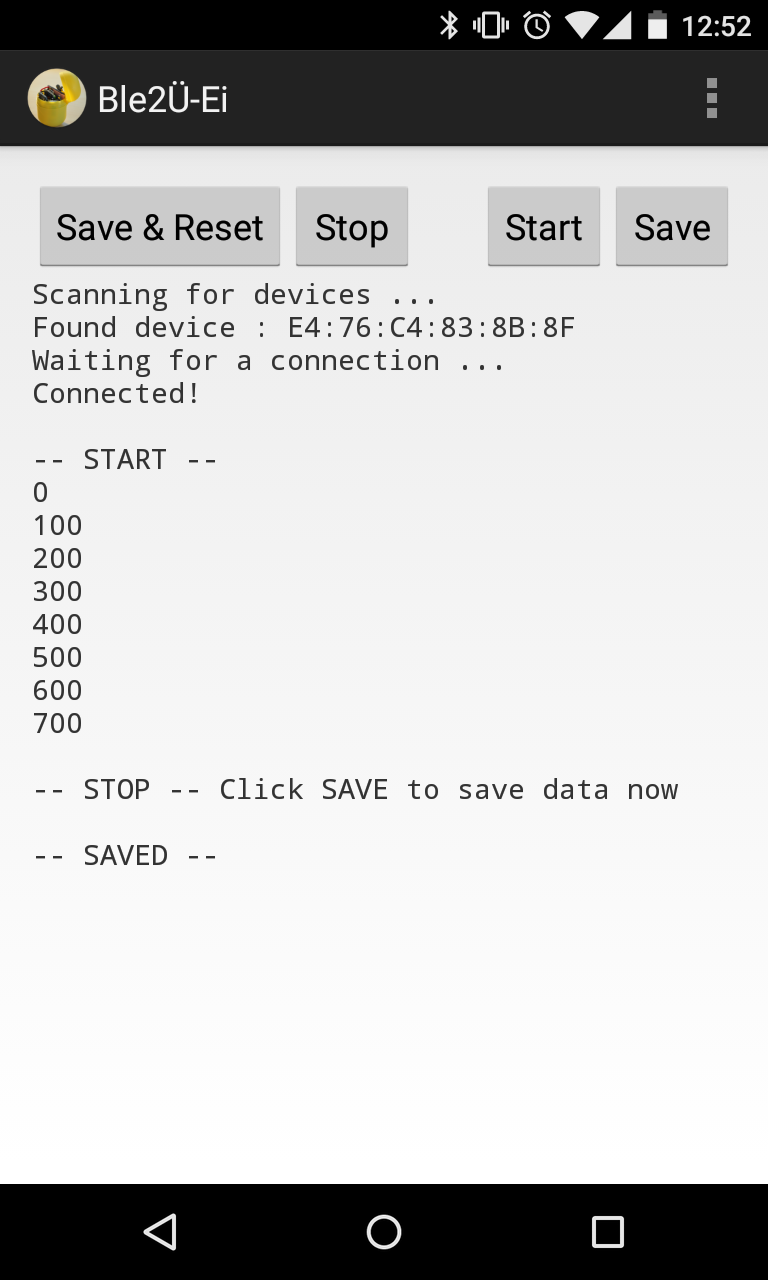
\includegraphics[width=0.5\textwidth]{images/k3-androidapp.png}
	\caption {Android-App zum Steuern des Mikrocontrollers und Empfangen der Sensordaten}
	\label{fig:k3_androidapp}
\end{figure}

Die Daten werden in Dateien lokal auf dem Smartphone gespeichert und müssen anschließend auf einen Rechner übertragen werden. Derzeit ist der ,,Download''-Ordner des Smartphones fest implementiert. Hier gibt es sicher noch Potential zur Erweiterung, indem die Daten direkt über einen Data Service an einen PC oder Laptop weitergeleitet werden oder zumindest der Speicherort selbst wählbar ist. \\
Abgelegt werden die Dateien in einem bestimmten Namensformat. Sie beginnen mit dem aktuellen Timestamp, um identische Dateinamen zu verhindern. Zusätzlich wird noch der Bereich mittels eines internen App-Zählers angegeben, um zusammenhängende Dateien für einen Messlauf identifizieren zu können.